\begin{figure}[t]
\tiny

%\fontfamily{lmss}\selectfont % Set font family to Latin Modern Sans Serif

\centering
\begin{tabular}
{ 
c@{\hspace{0.09cm}} c@{\hspace{0.09cm}} c@{\hspace{0.09cm}} c@{\hspace{0.09cm}} c@{\hspace{0.09cm}} c@{\hspace{0.09cm}} c@{\hspace{0.09cm}} c@{\hspace{0.09cm}} c@{\hspace{0.09cm}} c@{\hspace{0.09cm}}}
\toprule
    &
    \multicolumn{4}{c}{$\vcenter{\hbox{\textbf{Laysan albatross}}}$} &
    &
    \multicolumn{4}{c}{$\vcenter{\hbox{\textbf{Laysan albatross}}}$} \\
    
    &
    \multicolumn{4}{c}{ $\vcenter{\hbox{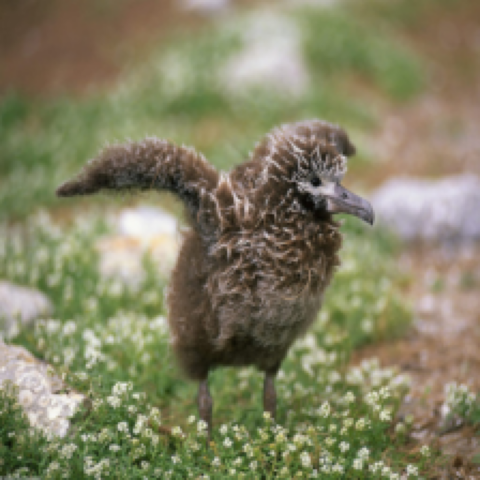
\includegraphics[width = 0.08\textwidth]{figures/Figure 5/42_true_1/input.png}}}$ } &
    &
    \multicolumn{4}{c}{$\vcenter{\hbox{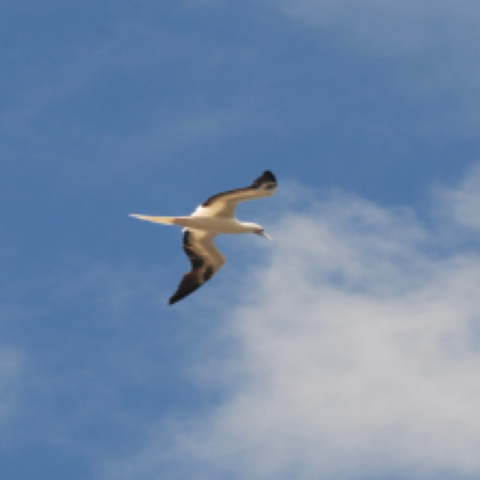
\includegraphics[width = 0.08\textwidth]{figures/Figure 5/34_true_1/input.png}}}$} \\

    &
    original &
    mean &
    max &
    weighted &
    &
    original &
    mean &
    max &
    weighted \\
    
    \vspace{0.09cm}
    $\vcenter{\hbox{\shortstack{Explanation for: \\ \textbf{Long-tailed jaeger} \\p=0.451}}}$ &
    $\vcenter{\hbox{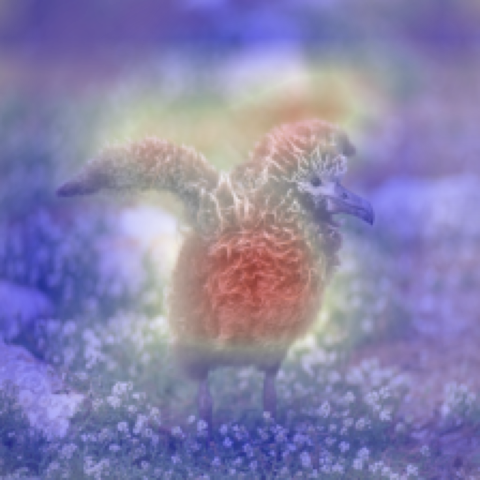
\includegraphics[width = 0.08\textwidth]{figures/Figure 5/42_true_1/original_GC_t1_70_0.451.png}}}$ &
    $\vcenter{\hbox{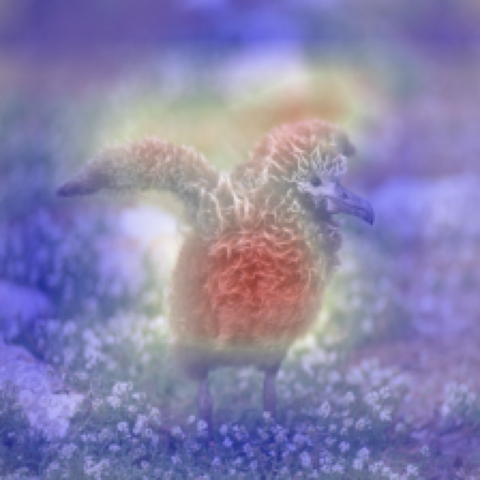
\includegraphics[width = 0.08\textwidth]{figures/Figure 5/42_true_1/mean_GC_t1_70_0.451.png}}}$ &
    $\vcenter{\hbox{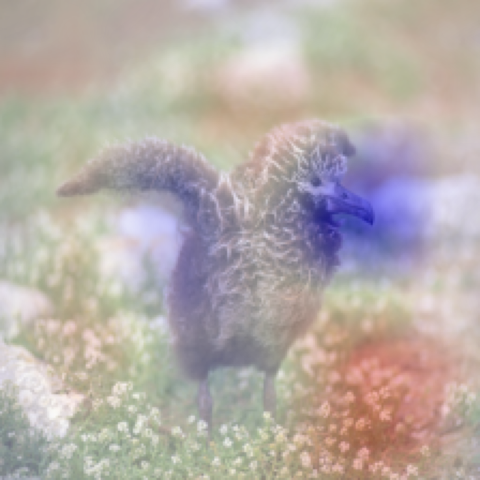
\includegraphics[width = 0.08\textwidth]{figures/Figure 5/42_true_1/max_GC_t1_70_0.451.png}}}$ &
    $\vcenter{\hbox{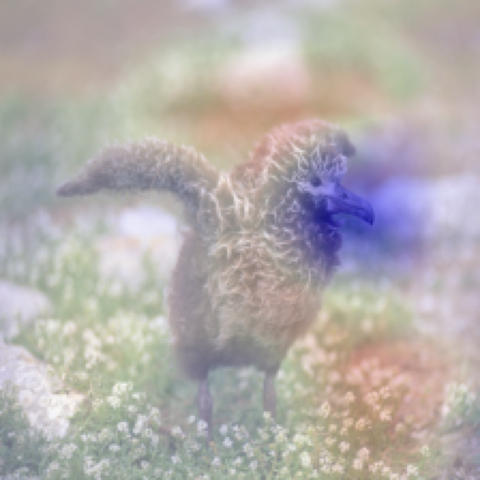
\includegraphics[width = 0.08\textwidth]{figures/Figure 5/42_true_1/weighted_GC_t1_70_0.451.png}}}$ &
    $\vcenter{\hbox{\shortstack{Explanation for: \\ \textbf{Sooty albatross} \\p=0.354}}}$ &
    $\vcenter{\hbox{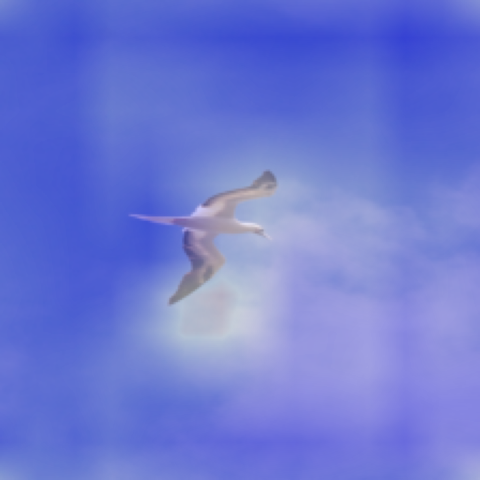
\includegraphics[width = 0.08\textwidth]{figures/Figure 5/34_true_1/original_GC_t1_2_0.354.png}}}$ &
    $\vcenter{\hbox{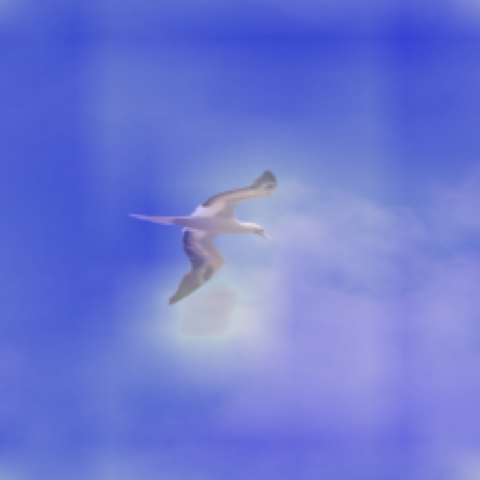
\includegraphics[width = 0.08\textwidth]{figures/Figure 5/34_true_1/mean_GC_t1_2_0.354.png}}}$ &
    $\vcenter{\hbox{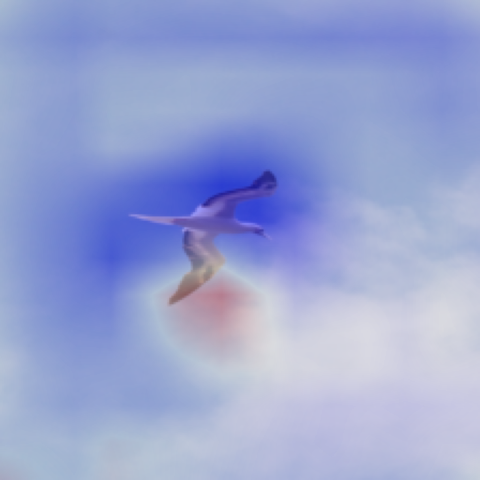
\includegraphics[width = 0.08\textwidth]{figures/Figure 5/34_true_1/max_GC_t1_2_0.354.png}}}$ &
    $\vcenter{\hbox{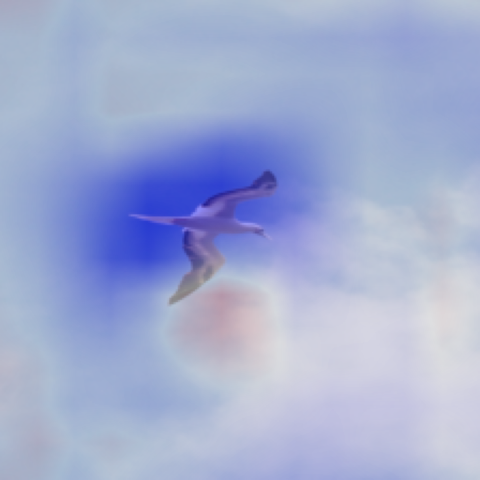
\includegraphics[width = 0.08\textwidth]{figures/Figure 5/34_true_1/weighted_GC_t1_2_0.354.png}}}$ \\

    \vspace{0.09cm}
    $\vcenter{\hbox{\shortstack{Explanation for: \\ \textbf{Laysan albatross} \\p=0.279}}}$ &
    $\vcenter{\hbox{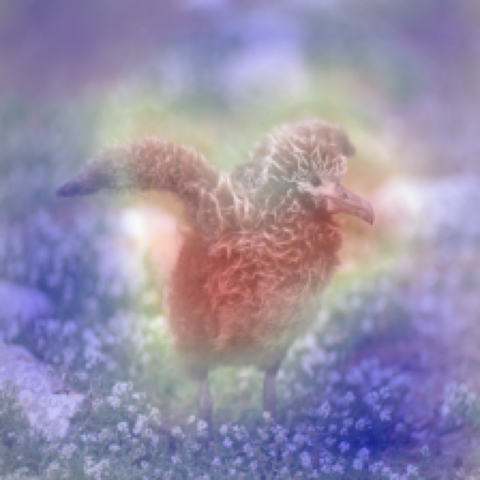
\includegraphics[width = 0.08\textwidth]{figures/Figure 5/42_true_1/original_GC_t2_1_0.279.png}}}$ &
    $\vcenter{\hbox{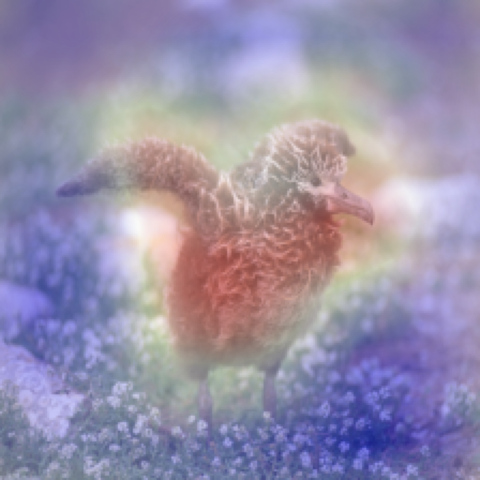
\includegraphics[width = 0.08\textwidth]{figures/Figure 5/42_true_1/mean_GC_t2_1_0.279.png}}}$ &
    $\vcenter{\hbox{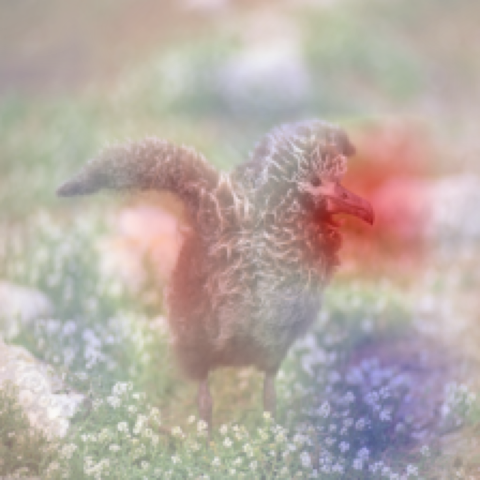
\includegraphics[width = 0.08\textwidth]{figures/Figure 5/42_true_1/max_GC_t2_1_0.279.png}}}$ &
    $\vcenter{\hbox{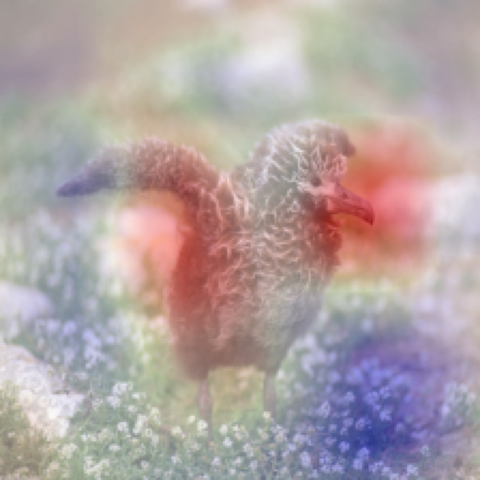
\includegraphics[width = 0.08\textwidth]{figures/Figure 5/42_true_1/weighted_GC_t2_1_0.279.png}}}$ &
    $\vcenter{\hbox{\shortstack{Explanation for: \\ \textbf{White pelican} \\p=0.214}}}$ &
    $\vcenter{\hbox{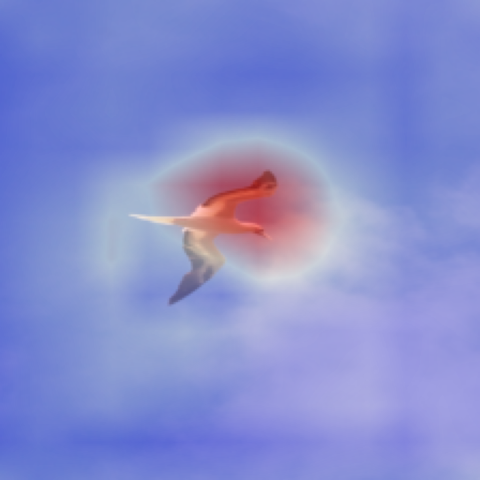
\includegraphics[width = 0.08\textwidth]{figures/Figure 5/34_true_1/original_GC_t2_100_0.214.png}}}$ &
    $\vcenter{\hbox{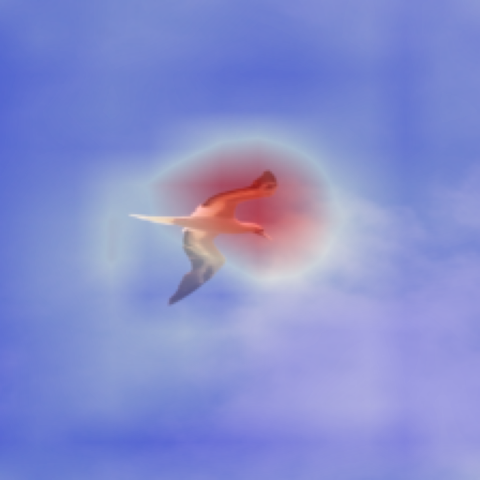
\includegraphics[width = 0.08\textwidth]{figures/Figure 5/34_true_1/mean_GC_t2_100_0.214.png}}}$ &
    $\vcenter{\hbox{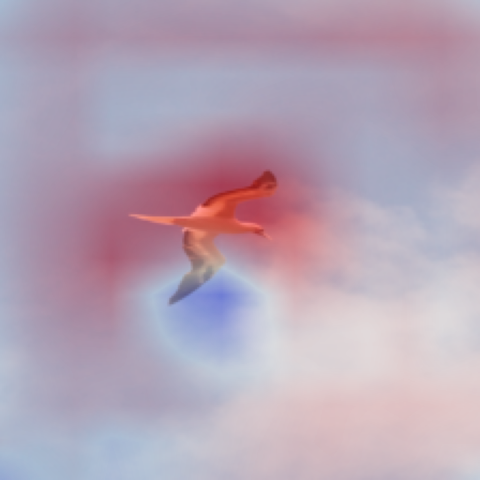
\includegraphics[width = 0.08\textwidth]{figures/Figure 5/34_true_1/max_GC_t2_100_0.214.png}}}$ &
    $\vcenter{\hbox{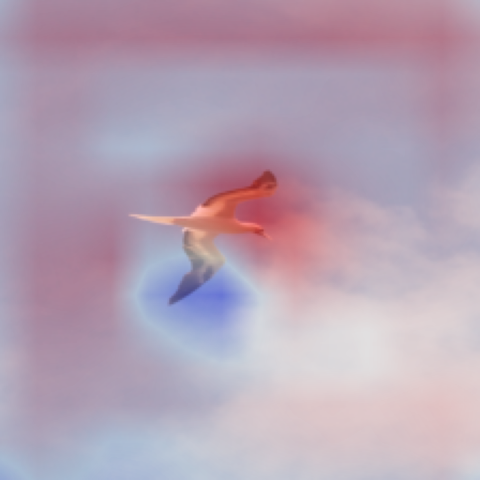
\includegraphics[width = 0.08\textwidth]{figures/Figure 5/34_true_1/weighted_GC_t2_100_0.214.png}}}$ \\
    \vspace{0.09cm}
    $\vcenter{\hbox{\shortstack{Explanation for: \\ \textbf{Geococcyx} \\p=0.134}}}$ &
    $\vcenter{\hbox{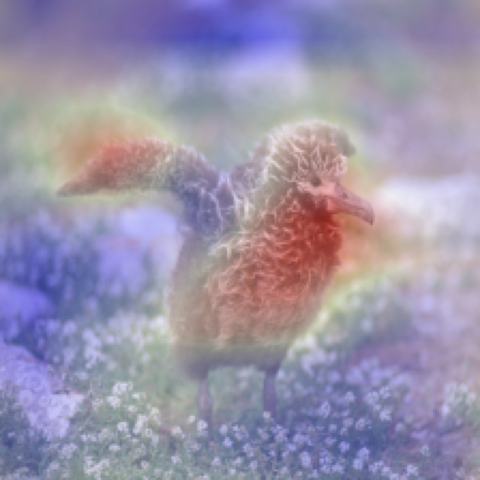
\includegraphics[width = 0.08\textwidth]{figures/Figure 5/42_true_1/original_GC_t3_109_0.134.png}}}$ &
    $\vcenter{\hbox{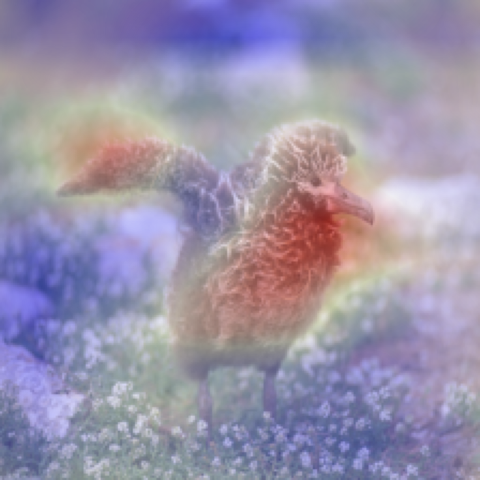
\includegraphics[width = 0.08\textwidth]{figures/Figure 5/42_true_1/mean_GC_t3_109_0.134.png}}}$ &
    $\vcenter{\hbox{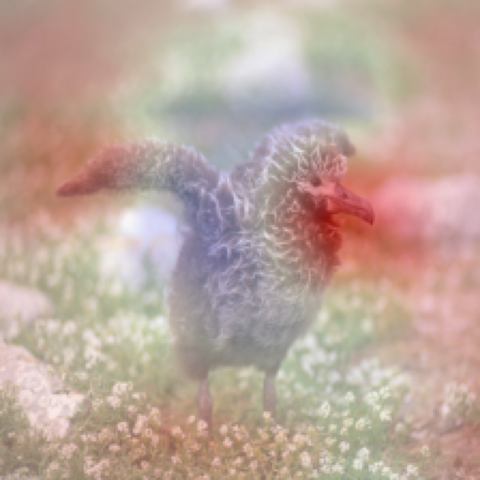
\includegraphics[width = 0.08\textwidth]{figures/Figure 5/42_true_1/max_GC_t3_109_0.134.png}}}$ &
    $\vcenter{\hbox{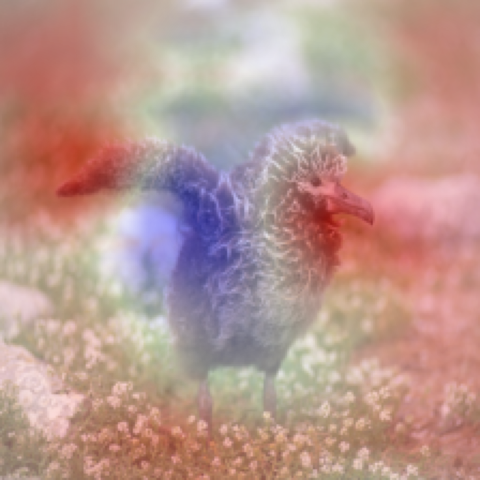
\includegraphics[width = 0.08\textwidth]{figures/Figure 5/42_true_1/weighted_GC_t3_109_0.134.png}}}$ &
    $\vcenter{\hbox{\shortstack{Explanation for: \\ \textbf{Frigatebird} \\p=0.194}}}$ &
    $\vcenter{\hbox{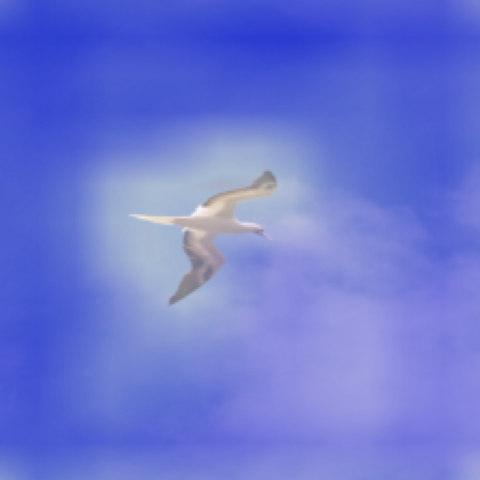
\includegraphics[width = 0.08\textwidth]{figures/Figure 5/34_true_1/original_GC_t3_43_0.194.png}}}$ &
    $\vcenter{\hbox{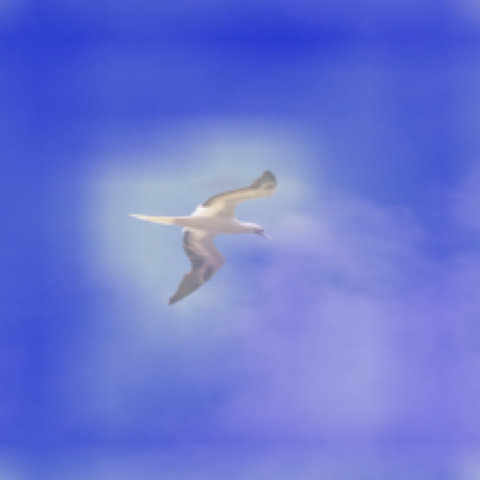
\includegraphics[width = 0.08\textwidth]{figures/Figure 5/34_true_1/mean_GC_t3_43_0.194.png}}}$ &
    $\vcenter{\hbox{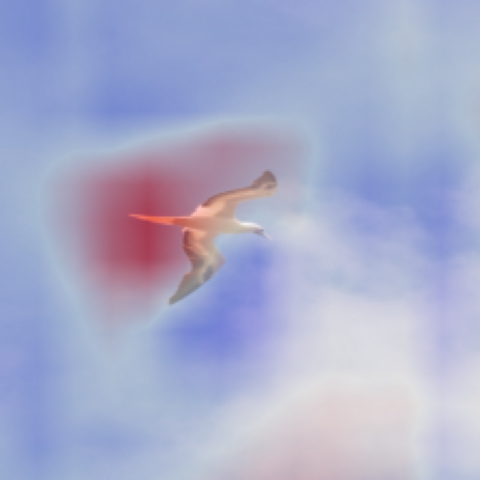
\includegraphics[width = 0.08\textwidth]{figures/Figure 5/34_true_1/max_GC_t3_43_0.194.png}}}$ &
    $\vcenter{\hbox{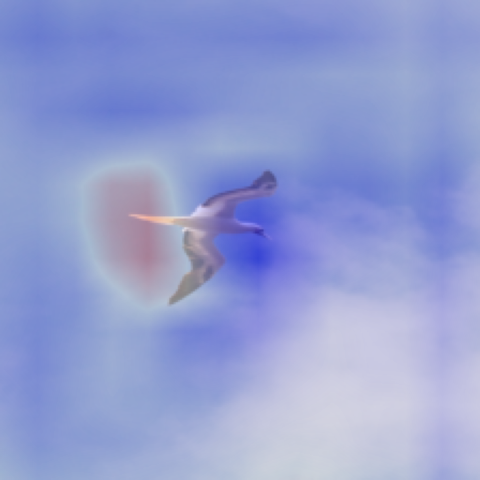
\includegraphics[width = 0.08\textwidth]{figures/Figure 5/34_true_1/weighted_GC_t3_43_0.194.png}}}$ \\

\midrule
    &
    \multicolumn{4}{c}{$\vcenter{\hbox{\textbf{Brewer blackbird}}}$} &
    &
    \multicolumn{4}{c}{$\vcenter{\hbox{\textbf{Eastern towhee}}}$} \\
    
    &
    \multicolumn{4}{c}{$\vcenter{\hbox{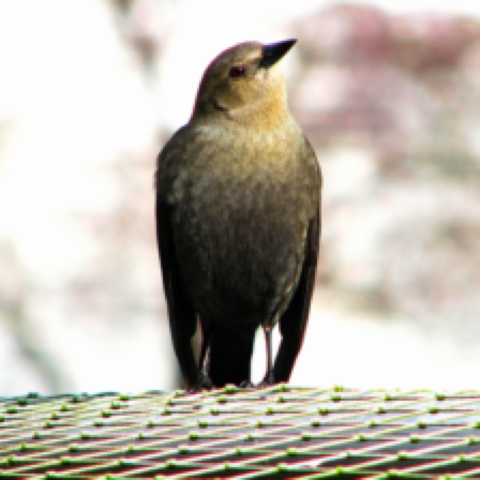
\includegraphics[width = 0.08\textwidth]{figures/Figure 5/194_true_8/input.png}}}$} &
    &
    \multicolumn{4}{c}{$\vcenter{\hbox{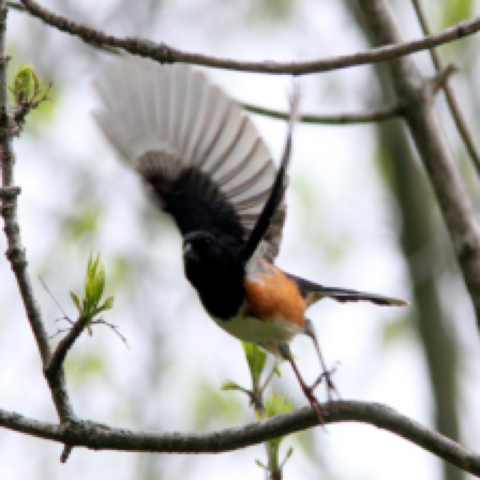
\includegraphics[width = 0.08\textwidth]{figures/Figure 5/542_true_20/input.png}}}$} \\

    &
    original &
    mean &
    max &
    weighted &
    &
    original &
    mean &
    max &
    weighted \\
    
    \vspace{0.09cm}
    $\vcenter{\hbox{\shortstack{Explanation for: \\ \textbf{American crow} \\p=0.334}}}$ &
    $\vcenter{\hbox{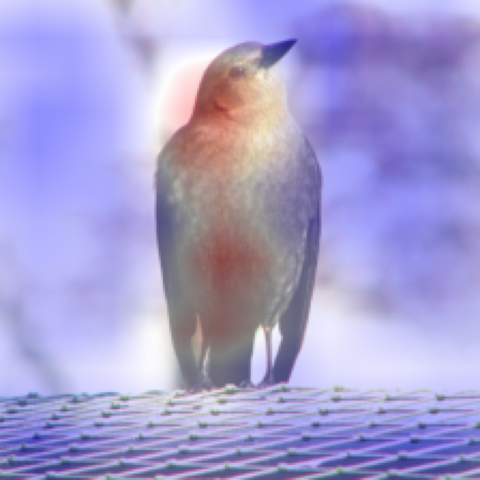
\includegraphics[width = 0.08\textwidth]{figures/Figure 5/194_true_8/original_GC_t1_28_0.334.png}}}$ &
    $\vcenter{\hbox{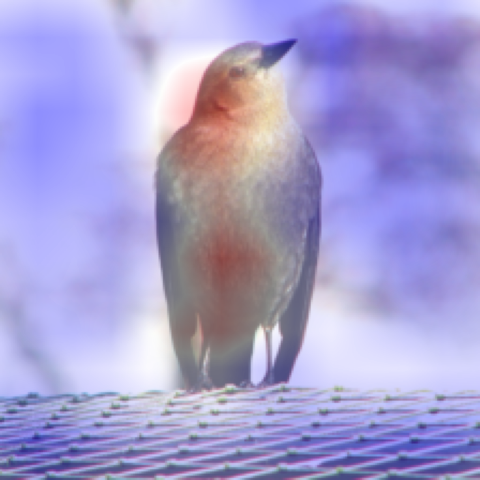
\includegraphics[width = 0.08\textwidth]{figures/Figure 5/194_true_8/mean_GC_t1_28_0.334.png}}}$ &
    $\vcenter{\hbox{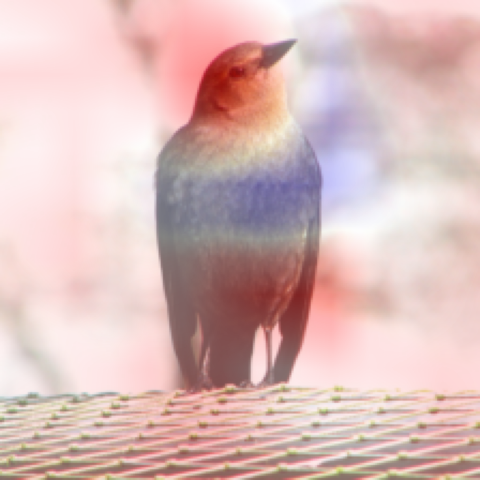
\includegraphics[width = 0.08\textwidth]{figures/Figure 5/194_true_8/max_GC_t1_28_0.334.png}}}$ &
    $\vcenter{\hbox{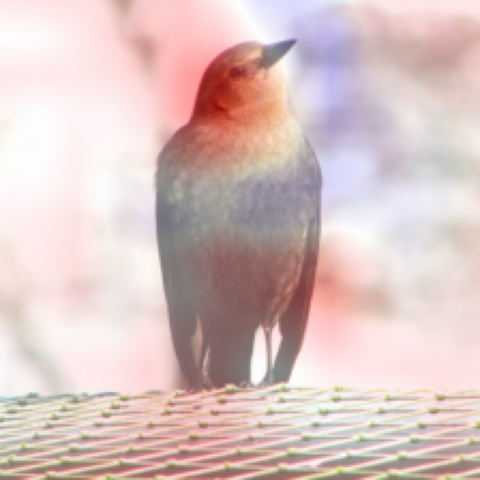
\includegraphics[width = 0.08\textwidth]{figures/Figure 5/194_true_8/weighted_GC_t1_28_0.334.png}}}$ &
    $\vcenter{\hbox{\shortstack{Explanation for: \\ \textbf{Orchard oriole} \\p=0.573}}}$ &
    $\vcenter{\hbox{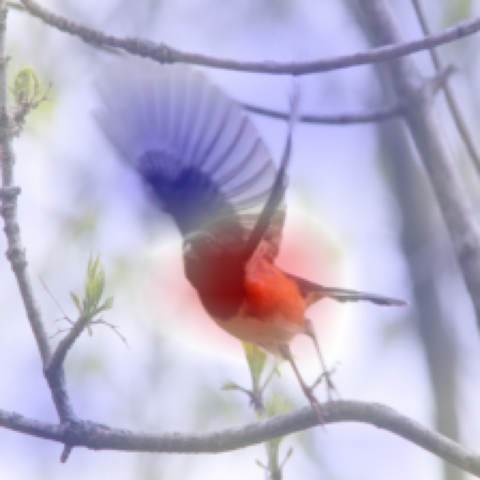
\includegraphics[width = 0.08\textwidth]{figures/Figure 5/542_true_20/original_GC_t1_96_0.573.png}}}$ &
    $\vcenter{\hbox{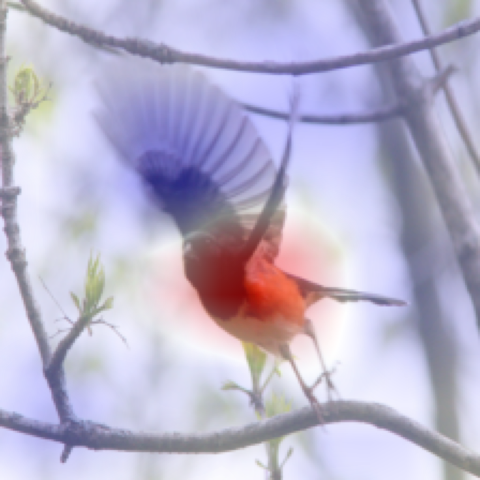
\includegraphics[width = 0.08\textwidth]{figures/Figure 5/542_true_20/mean_GC_t1_96_0.573.png}}}$ &
    $\vcenter{\hbox{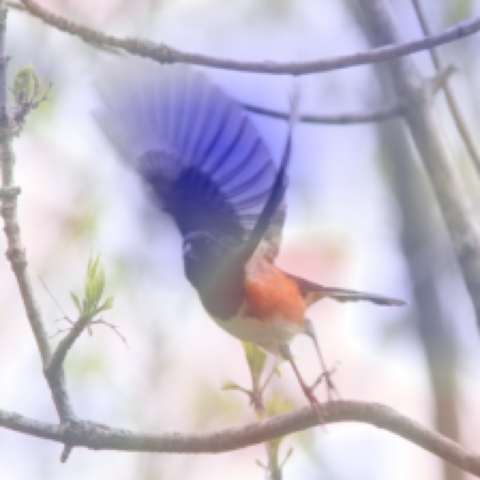
\includegraphics[width = 0.08\textwidth]{figures/Figure 5/542_true_20/max_GC_t1_96_0.573.png}}}$ &
    $\vcenter{\hbox{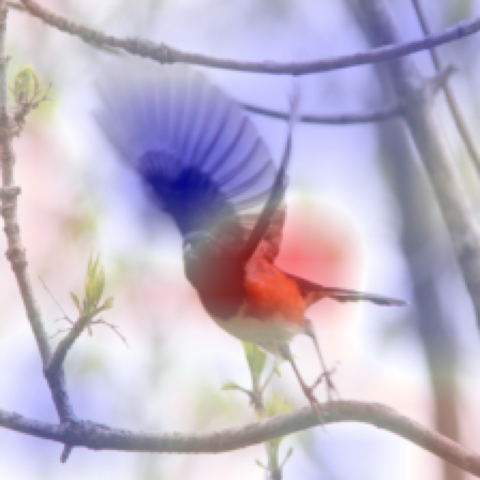
\includegraphics[width = 0.08\textwidth]{figures/Figure 5/542_true_20/weighted_GC_t1_96_0.573.png}}}$ \\

    \vspace{0.09cm}
    $\vcenter{\hbox{\shortstack{Explanation for: \\ \textbf{Crested auklet} \\p=0.310}}}$ &
    $\vcenter{\hbox{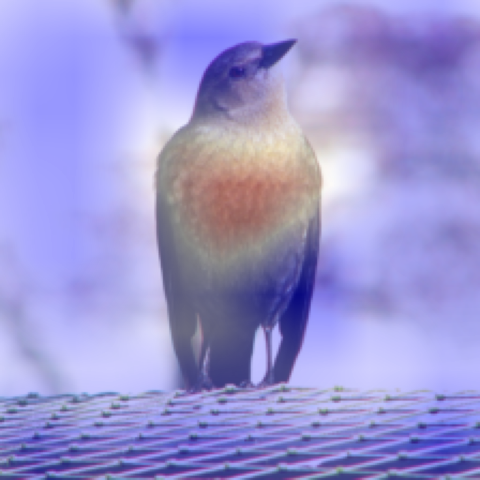
\includegraphics[width = 0.08\textwidth]{figures/Figure 5/194_true_8/original_GC_t2_4_0.310.png}}}$ &
    $\vcenter{\hbox{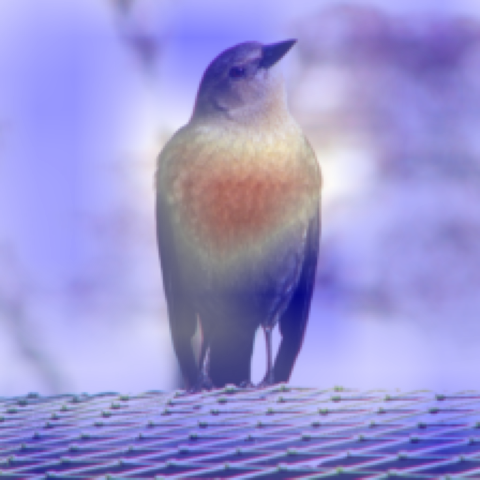
\includegraphics[width = 0.08\textwidth]{figures/Figure 5/194_true_8/mean_GC_t2_4_0.310.png}}}$ &
    $\vcenter{\hbox{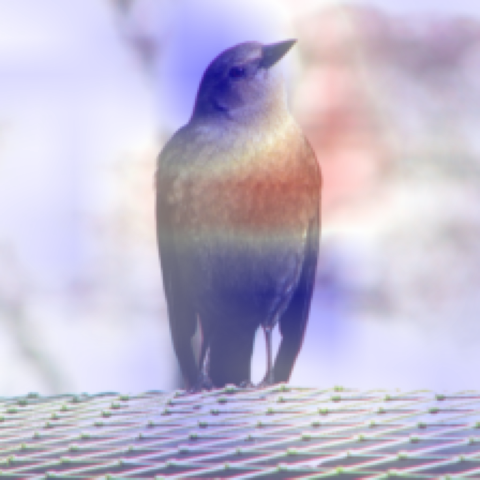
\includegraphics[width = 0.08\textwidth]{figures/Figure 5/194_true_8/max_GC_t2_4_0.310.png}}}$ &
    $\vcenter{\hbox{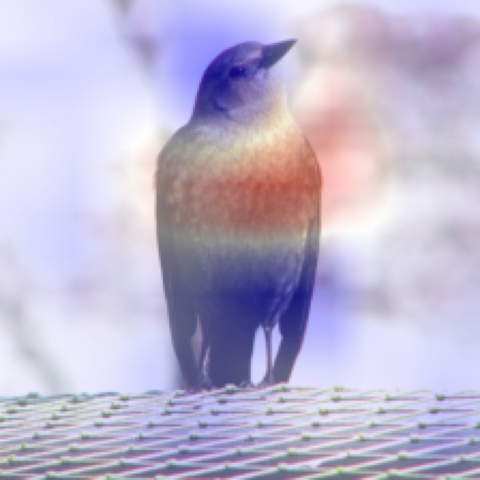
\includegraphics[width = 0.08\textwidth]{figures/Figure 5/194_true_8/weighted_GC_t2_4_0.310.png}}}$ &
    $\vcenter{\hbox{\shortstack{Explanation for: \\ \textbf{Baltimore oriole} \\p=0.141}}}$ &
    $\vcenter{\hbox{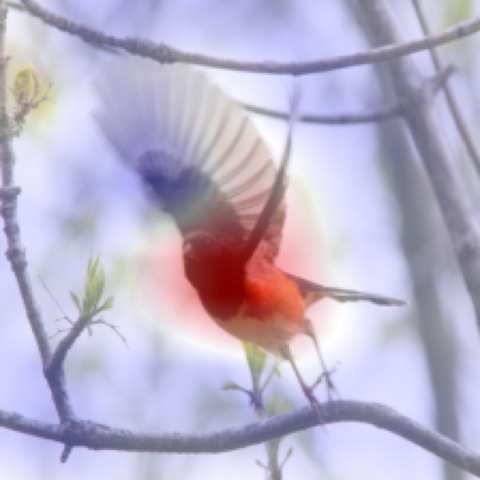
\includegraphics[width = 0.08\textwidth]{figures/Figure 5/542_true_20/original_GC_t2_94_0.141.png}}}$ &
    $\vcenter{\hbox{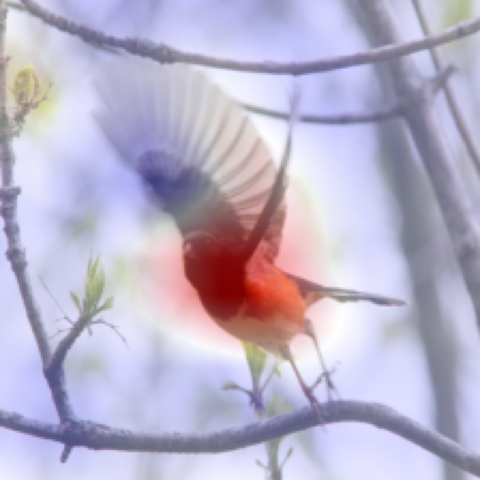
\includegraphics[width = 0.08\textwidth]{figures/Figure 5/542_true_20/mean_GC_t2_94_0.141.png}}}$ &
    $\vcenter{\hbox{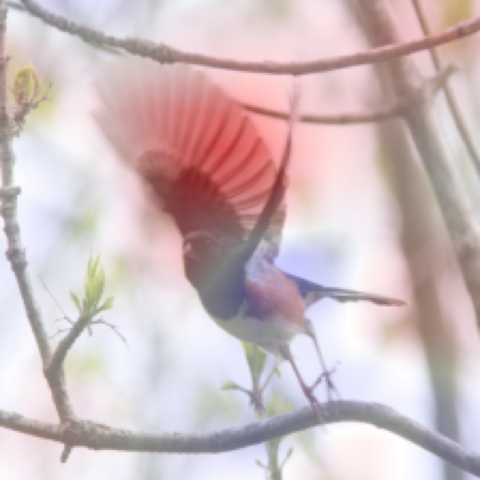
\includegraphics[width = 0.08\textwidth]{figures/Figure 5/542_true_20/max_GC_t2_94_0.141.png}}}$ &
    $\vcenter{\hbox{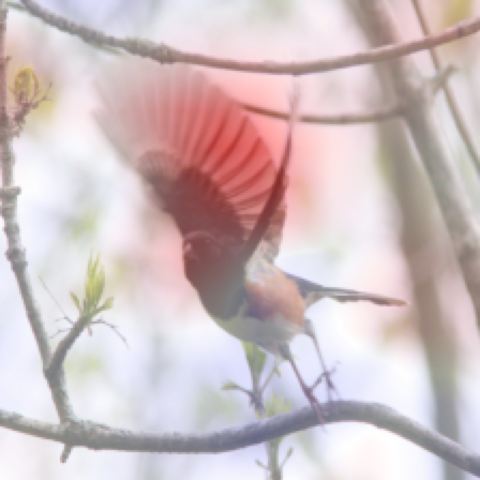
\includegraphics[width = 0.08\textwidth]{figures/Figure 5/542_true_20/weighted_GC_t2_94_0.141.png}}}$ \\

    \vspace{0.09cm}
    $\vcenter{\hbox{\shortstack{Explanation for: \\ \textbf{Red-winged blackbird} \\p=0.110}}}$ &
    $\vcenter{\hbox{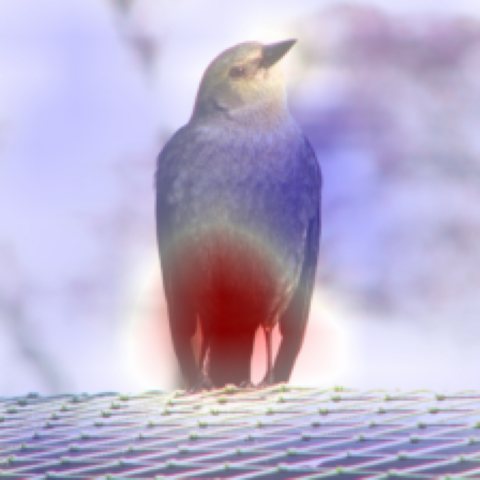
\includegraphics[width = 0.08\textwidth]{figures/Figure 5/194_true_8/original_GC_t3_9_0.110.png}}}$ &
    $\vcenter{\hbox{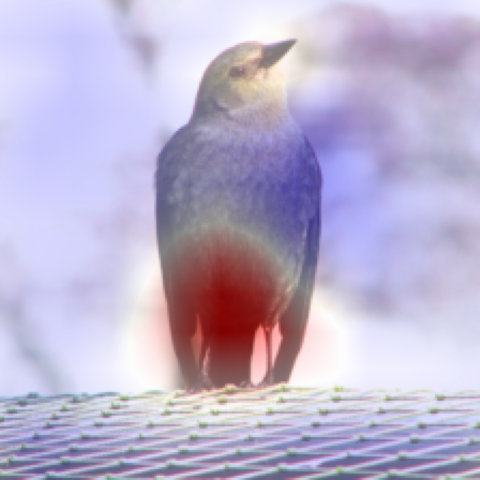
\includegraphics[width = 0.08\textwidth]{figures/Figure 5/194_true_8/mean_GC_t3_9_0.110.png}}}$ &
    $\vcenter{\hbox{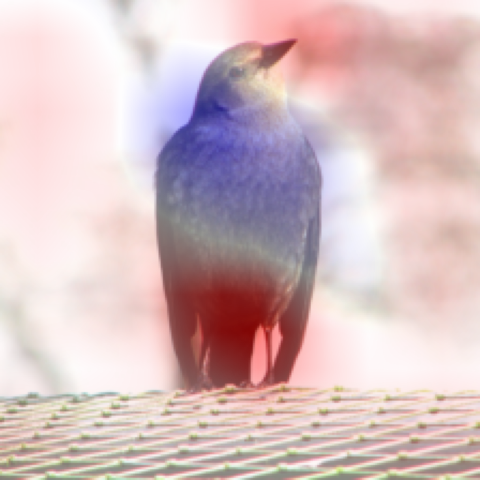
\includegraphics[width = 0.08\textwidth]{figures/Figure 5/194_true_8/max_GC_t3_9_0.110.png}}}$ &
    $\vcenter{\hbox{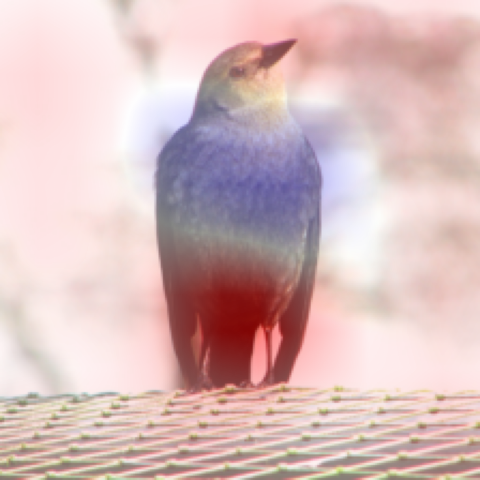
\includegraphics[width = 0.08\textwidth]{figures/Figure 5/194_true_8/weighted_GC_t3_9_0.110.png}}}$ &
    $\vcenter{\hbox{\shortstack{Explanation for: \\ \textbf{American redstart} \\p=0.130}}}$ &
    $\vcenter{\hbox{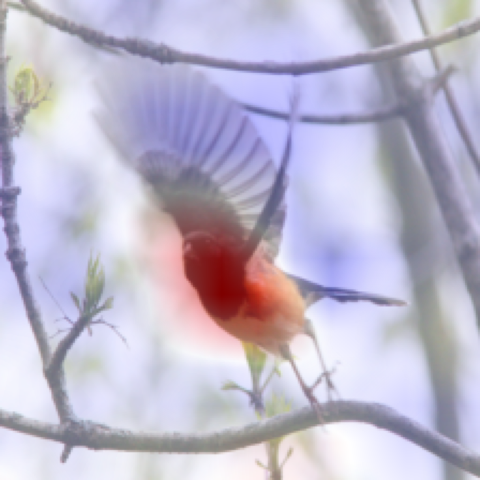
\includegraphics[width = 0.08\textwidth]{figures/Figure 5/542_true_20/original_GC_t3_108_0.130.png}}}$ &
    $\vcenter{\hbox{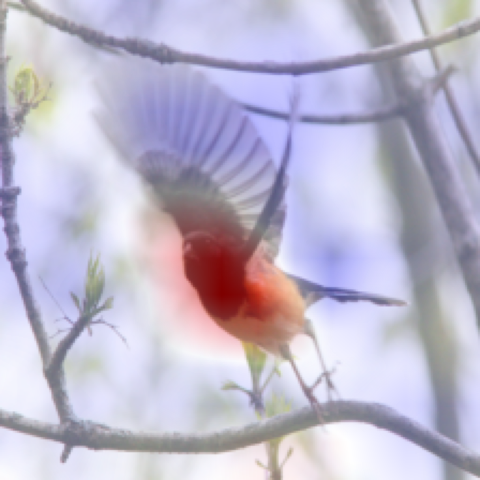
\includegraphics[width = 0.08\textwidth]{figures/Figure 5/542_true_20/mean_GC_t3_108_0.130.png}}}$ &
    $\vcenter{\hbox{\includegraphics[width = 0.08\textwidth]{figures/Figure 5/542_true_20/max_GC_t3_108_0.130.png}}}$ &
    $\vcenter{\hbox{\includegraphics[width = 0.08\textwidth]{figures/Figure 5/542_true_20/weighted_GC_t3_108_0.130.png}}}$ \\

    

\bottomrule
\end{tabular}
\caption{Reproduction of Figure 5 in the original paper. Comparison between mean, max, and weighted contrast for four images from CUB-200. In each column, we present explanations for the three most probable classes for GradCAM using the original image and the three contrastive methods.} \label{f:meanmaxcomp}
\end{figure}